%!TEX root = ../Thesis.tex
\chapter{Interpretation of random forest models}

\section{Modeling with random forest}
The random forest model started to play a bigger role for this thesis as it showed to outperform linear regularized regression models as partial least squares and elastic net. Also RF seem to outperform the non-linear k-nearest neighbor. The random forest algorithm is certainly not always the best choice of a model, the non free lunch theorem states that there is no optimal silver bullet. That said Random forest together with radial support vector machine and gradient boosting was in comparison on 110 data sets found to be the in generel top performing algorithm in terms of cross-validated accuracy \cite{wainer2016comparison}. If the underlying model generating the data is truly linear, e.g. in octane concentration determination in near-infrared light spectroscopy \cite{kalivas1997two}, then linear regression well perform better than random forest.


\section{One interpretation of interactions}
\label{defineInteractions}
Throughout the work of this thesis, there have been an emphasis on identifying and visualizing interactions. In this process, I have developed my own definitions of interactions, that especially relate to geometrical interpretations of model structures. In our paper \textit{Forest Floor Visualizations of Random Forests} we introduce an interaction as:

\begin{quotation}
\textit{
"Interactions in the model structure mean that the model predictions in part rely on the interplay on two or more features. Thus, the interaction parts of a model structure cannot be reduced to additive scoring rules, one for each feature. Likewise, to plot single feature-to-prediction relationships is not a sufficient context for visualizing any interactions."
}
\cite{welling2016forest}
\end{quotation}

I would like to elaborate on this definition of interactions. First definitions of the model structures, feature spaces and prediction spaces are needed. A given model structure
\footnote{Throughout Chapter \ref{chap_introStat}, $f$ has referred to the underlying function to match the notation of Figure \ref{modelPredictExplain}\cite{Mostafa2013learning}. However, in this chapter $f$ refers to the model structure to match the notation of the forestFloor article \cite{welling2016forest}.}
$f$ maps from feature space $X$ to a prediction space $\hat{y}$, such that $\hat{y} = f(X)$. $X$ is a real valued euclidean vector space, constituted by $d$ axes $x_1$,...,$x_d$. Any point is a unique combination of feature values.
\footnote{See the forestFloor article \cite{welling2016forest} or this how to handle categorical features, an idea originally from Friedmans gradient boosting and partial dependence article \cite{friedman2001greedy}.}
For regression the prediction space $\hat{y}$ is simply an one-dimensional real axis. We understand $f$ as a function which connect any point in the feature space to some point in prediction space. To discuss how to describe interactions, I will introduce a simple structure. We can imagine the surface of a regression function $f$ in a Eucledian 3D space, for two features $x_1$ and $x_2$ spanning the horizontal plane and one vertical prediction axis. We call this joint feature space and prediction space for the mapping space. We can imagine the structure of $f$ is a geographical landscape model of altitude as function of coordinates. This $f$ mapping has potentially valleys and mountains. Essentially, if $f$ can be reduced into separate additive score functions, we can for any ($x_1$,$x_2$) coordinate position in this landscape not only use $f$ to calculate the altitude, but also $f$ decomposed into $f_1$ and $f_2$, such that $\hat{y} = f(X) = f_1(x_1) + f_2(x_2)$. When the mapping space is only 3D, it is not obvious, why we want to decompose $f$. However, for higher dimensional models, we cannot directly visualize nor comprehend the geometrical structure. By decomposing the model structure we allow ourselves to split the full structure in to simpler pieces we can visualize and understand. Unfortunately not all landscapes can be reduced to such additive scoring rules. Returning to the altitude model $f$, imagine a landscape model of a single pyramid surrounded by a flat dessert, see Figure \ref{pyramid}. A function describing the local height of this landscape would reflect, that only when $x_1$ AND $x_2$ match the position of the pyramid, then the predicted altitude should rise above the sands. To decompose this topological map into $f_1$ + $f_2$ would analogously correspond to two observers on either side of the pyramid, where neither can see the entire pyramidn but only their respective front sides. Either observer would notice that in the middle of their respective fields of view, the altitude is elevated due to the pyramid. Each observer could generalize what they see to a partial function parallel to their field of view. However, as they cannot see their back side of the pyramid, neither of the observers will know if this is generally true for any position on the other axis. If we simply combined by averaging the altitude predictions of the two naive observers, the model structure would more look like the roof of a tower, not a pyramid. 

\begin{figure}
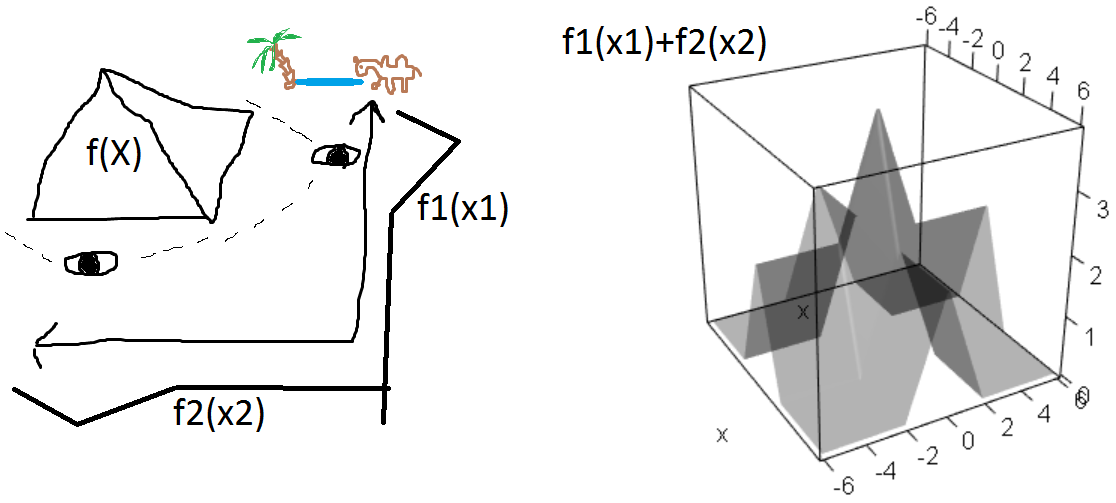
\includegraphics[width=\textwidth,height=\textheight,keepaspectratio]{graphics/sketch_pyramid_interaction.png}
\caption{Left, pyramid in flat sands, an example of a model structure with non-global non-saddle interaction. XY-plane describes the coordinates. Z-axis is the altitude. Two naive observers f1 and f2 cannot approximate the shape of the pyramid alone. Right, approximated shape of the pyramid if f1 and f2 are combined additively.}
\label{pyramid}
\end{figure}

In the mini review (letter) of boulesteix \textit{et al} points out that the definition of interations can be vague and ambiguous in recent litterature \cite{boulesteix2014letter}. They refer to the simple classical statistical logit-model, that contains a well defined two-feature saddle point interaction. Here $f$ is decomposed such that $\hat{y} = f(X) = P(\beta_1 x_1 + \beta_2 x_2 + \beta_{12} x_1 x_2)$ where $P$ is the logit transfer function $P(z) = log(\frac{z}{1-z})$. The logit function is used to let $\hat{y}$ describe the probability of some binary outcome. We could generalize and say $P$ could be any polynomial function. An interaction term stated as the product of two features is called a saddle point structure, as the shape resembles a saddle. Even when the product of two features is wrapped in a transfer function $P$, this interaction is a saddle point. The transfer function $P$ can be seen as a compression/rearrangement of the $\hat{y}$ prediction axis. The limitation of the saddle point structure is that it can neither fit the shape of the pyramid, because the pyramid is a local interaction in an otherwise flat dessert sand landscape. My postulate is that there is no combination of compressing, stretching or looping of the $\hat{y}$ axis, which can morph a saddle point structure into the pyramid structure. Therefore, I postulate that logistic models comprised by the coefficient weighted sum of main effects and a number of saddle point interactions and any transfer function $P$ is not a suitable basis for decomposing any model structure. There are structures, which do not fit this scheme. For any $f_{12}$ there is not necessarily a $P$ such that $f_{12}(x_1,x_2) = P(\beta x_1+ \beta x_2 + \beta_{12} x_1 x_2$. 

To decompose any possible landscape, including the pyramid, let 
$f(X)= f_1(x_1) + f_2(x_2) + f_12(x_1,x_2)$. If $f_{12} = f$ then not much have been accomplished. In fact their are a lot of really unuseful decompositions of $f$. In general it would be helpful to describe as much of the structure as possible as additive main effects and only what absolutely necessary as a higher order interaction. Let us imagine the pyramid is placed in a landscape steadily descending towards a ocean. Then the $f_1$ and/or $f_2$ can describe this general descending trend, while $f_12$ describe the pyramid.

A non-linear regression model of $d$ features can be decomposed into bias/offset, $d$ main effects, $d-1$ second order effects, and a number of higher order effects. The type of decomposition we aim for is one, that explains as much of the structural features in lower order effects. In the following, I derive that the number of possible components approximately doubles per feature.

For a model of $d$ features there will be effects of $d$ different orders. The smallest of first order (main effect) and the highest of $d^{th}$ order. The number of combinations to draw $i$ features in a $d$-features can be described as binomials. Summing all binomial counts from $i=1$ to $d$ give the number possible components/effects of the system. Therefore, $n_d$ the number of possible effects are calculated as, 
$n_d = \sum_{i=1}^{d} \binom{i}{d}$. Furthermore the number $n_d$ can be defined by $n_{d-1}$ as,
$n_d = 2n_{d-1} + d$. For $d=10$ there are staggering $2036$ possible components effects. Suddenly one may get sweaty hands, when to learn there are so many different effects of a multivariate model with 10 features. The promise that decomposition of the model structure would bring simplicity and clarity seems far from fulfilled. Fortunately, we can ignore a high number of these components when emphasizing model structures trained by random forest or any other reasonable machine learning algorithm. As shown in supplementary materials for the forest floor article, random forest can only poorly fit a saddle point interaction of 3 orders and 4 orders are nearly impossible. We live in a reality where fifth order interactions always will be near impossible to robustly estimate with statistical models and finitely sized training sets. Adhering to the Occam's Razor guideline, that we should always pick the simplest model explaining the observed data, all effects of more than 2 or 3 orders can in practice be disregarded. Furthermore, a subset of features will often be used more frequently than others in splits in the trees of the random forest. Interactions terms can only be learned in a tree model, when one split by one feature is conditioned by another feature split upstream. As the most dominant features tend be the ones upstream, interactions in the model structure are most likely found in the model structure as second order interactions between one relatively dominant feature (high variable importance) and some other feature. Therefore, interactions between weak features can be disregarded at first. Therefore, the a random forest model can be decomposed into $d$ main effects and a lower number of second order effects, where at least one feature likely have been the favorite splitting feature. To summarize, an interaction effect of $i^th$ order is one that cannot be fully be described by any combination of lower order effects.

This broad definition of interaction effects can also cover classification and multi classification, where $f$ map to a $K-1$ dimensional simplex probability space, where $K$ is the number of classes. Second order interaction effects for a probabilitic classification model mapping to 3 classes($K=3$) are visualized in the forest floor article, see figure 12 \cite{welling2016forest}. However, the surface of this second order interaction effect is not 3 dimensional as the pyramid example. For a second order interactions($i=2$), the mapping space has $i+K-1=2+3-1=4$ dimensions. In the forest floor article a such 4D problem is visualized in Figure 12. Here a 2D triangular (K-1)-simplex diagram is used to describe the probability distribution of predictions, and different color gradients in turn represent the different feature axes. 
\footnote{If number of classes $K>=5$ is higher than 5, the (K-1)-simplex diagram would require a 4D or higher visualization. Instead Figure 10 of article depicts how to plot probability predictions by each class by a single axis.}

Returning to pyramid example. Let's say $f_1$ described the gradual descending of the landscape towards the ocean. As $f_1$ is non-linear, it could describe a single sand dune, a local maximum, parallel to the beach. This local sand dune now have to stretch infinitely to both sides, such that for any $x_2$ the effect of $f_1$ is static. We can use this observation to make a bottom up definition of interactions also. Let $S$ be a subset of all features $X$ of the model. Let $T$ bet the complimentary subset of features. An interaction effect by subset $S$, $f_S$, has the order equal to size of $|S|$. We would know that $f_S$ is an adequately detailed decomposition of $f$, as for every parallel plane spanned by the features in $S$, the curvature of $f_S$ align with $f$. In contrary when the interaction curvature is far from the same by any combination of feature vales of $T$, we know we are missing an important interaction with some feature(s) from $T$. Furthermore, that feature of $T$, by which the $S$-plane curvature changes the most, is the one that need to be included in $S$, in order to obtain a better generalized effect. This bottom up definition of interaction effects lend it notion of complimentary feature subsets $S$ and $T$ from Friedmans paper on gradient boosted machines and partial dependence plots \cite{friedman2001greedy}. What I effectively state here is, that if a partial dependence plot of subset $S$ is a poor generalization of $f$, then an interaction with one or more features from $T$ are missing. 

\section{Article 3: \textit{Forest Floor Visualizations of Random Forests}}
\label{article:forest}
First version submitted to arXiv.org the 30$^{th}$ of May 2016.
Latest version (3$^{rd}$) submitted to arXiv.org the 4$^{th}$ of July 2016.

\newpage
\includepdf[pages={1-},scale=0.90,pagecommand={\pagestyle{myruled}}]{chapters/forestFloorArt.pdf}

\subsection{Supplementary materials for: Forest Floor Visualizations of Random Forests}
\label{forestFloorSuppl}

\includepdf[pages={2-},scale=0.90,pagecommand={\pagestyle{myruled}}]{chapters/supplementaryForestFloor.pdf}